\chapter{Introduction:}

Anthropogenic climate change is the product of human activities \citep{trenberth2018climate} that have been implemented since the \ac{ir} and that have strongly intensified in recent decades. Among other effects, global warming results from the increasing concentration of heat-trapping \ac{ghg} in the atmosphere mainly due to fossil fuel burning, which causes global temperatures to rise. This and other climatic alterations heavily affect local communities and natural ecosystems around the world, leading to "severe, pervasive and irreversible impacts" \citep{change2014impacts}.

According to most projections, the \ac{pa} to keep global temperatures well below 2\textdegree C, and possibly below 1.5\textdegree C, compared to pre-industrial levels, is unlikely to be realised by the end of the century only by reducing \ac{ghg} emissions. In fact, most model predictions show that existing commitments are inadequate to meet such targets \citep{lawrence2018evaluating}. The \ac{ipcc} report drawn up by the Working Group III reinforces this evidence by stating that national unconditional commitments determine a global warming far beyond \ac{pa} standards and that human manipulation of the earth’s climate is necessary to offset hard-to-abate emissions \citep{IPCC_2022_WGIII_SPM}.

As \ch{CO2} is one of the most potent \ac{ghg} contributing to the earth's warming, \ac{cdr} is being investigated as part of the \ac{pa}-driven collaborative mission to achieve climate mitigation. The aim of this technique is to relieve the atmosphere from \ch{CO2}-induced pollution and reach net negative emissions by 2100. Therefore, this research focuses on an example of marine \ac{cdr}, that is, carbon dioxide sequestration and storage in oceanic reservoirs, termed \ac{oae}. This method aims to enhance surface ocean alkalinity through accelerated chemical weathering of mineral rocks or solutions in order to reduce ocean \ch{CO2} partial pressure (\ch{pCO2}) and increase the ocean's uptake potential. 

For this manuscript, output data from two \ac{esm} simulations were analysed, projecting future scenarios with and without alkalinity applied to the European coastline (excluding the Baltic and the Mediterranean seas) for a low and a high emission scenario (SSP1-2.6 and SSP3-7.0, respectively). The purpose was to understand the effects of \ac{oae} on the carbon cycle and, particularly, on its seasonal variations, as seasonality is a fundamental component regulating the annual net carbon flow at the air-sea interface.

This paper develops as follows. First, the study objectives and hypotheses are formulated. The second chapter aims to illustrate the present-day relevance of marine \ac{cdr}, and especially of \ac{oae}, and describe the factors that drive \ch{CO2} flux and ocean \ch{pCO2} seasonality, both globally and in the study area. In the third chapter, the methods are presented, giving a description of the \ac{esm} and of the simulations utilised for this manuscript, together with a brief overview of the addressed variables. The results are provided in the fourth chapter. The fifth chapter includes a discussion section, which outlines the possible causes behind the findings, and the sixth highlights the study's limitations and some key recommendations for future research. 

\section{Study objectives and hypothesis formulation:}

As the \ac{pa} targets become increasingly difficult to attain, the employment of \ac{cdr} to counterbalance hard-to-abate emissions is considered a future necessity \citep{IPCC_2022_WGIII_SPM, shukla2022summary}. Despite being a potentially significant contribution to climate mitigation, \ac{oae}, one of the proposed marine-\ac{cdr}, is still widely unexplored \citep{fakhraee2022environmental}. Thus, more research is needed to shed light on the impacts of \ac{oae} on the cycle of \ch{CO2} and ocean \ch{pCO2} at the air-sea interface. This is the case especially for coastline alkalinity addition, where such highly dynamic environments are thought to be particularly favourable to accelerated carbon sequestration \citep{he2022limits, thomas2009enhanced}. 

Seasonality is one of the fundamental elements influencing the net annual \ch{CO2} cycle. Understanding how such patterns will evolve with large-scale \ac{oae} implementation is therefore relevant for a variety of reasons. First, if changes to the seasonal carbon cycle are not counterbalanced by compensating effects in the opposite direction, these asymmetries may trigger significant modifications to the annual net cycle \citep{fassbender2022quantifying}. Furthermore, \ch{CO2} flux seasonality is a central driver of ocean extreme events such as earlier calcium carbonate undersaturation \citep{kwiatkowski2022modified} and intensified ocean acidification \citep{sasse2015quantifying}, other than acting upon inter-annual variability patterns \citep{rustogi2023impact}. Lastly, while atmospheric \ch{pCO2} responds to system stimuli at much shorter timescales, the ocean can take several seasons to react \citep{salt2013variability} and defining such time lapses is necessary for future \ac{oae} application.

Thus, up to this day, uncertainty remains on how \ac{oae} would affect \ch{CO2} seasonality and what patterns it would follow under different future climatic conditions. The main research questions that were formulated to address this knowledge gap are:
\begin{enumerate}

  \item How will \ac{oae} modify the \ch{CO2} flux and ocean \ch{pCO2} seasonal cycle in European waters?:
  \item What are the main physical and biological drivers of such system alterations?
  \item What role does the future emission scenario play in the seasonality of \ch{CO2} flux and ocean \ch{pCO2} when \ac{oae} is implemented?
  
\end{enumerate}

A 2022 report by \cite{schwinger2022report} pictured an idealised simulation of global \ac{oae} application to account for seasonal implications of \ch{CO2} flux and other variables. Results showed that \ac{oae} has the potential to increase the \ch{CO2} seasonal cycle, elicited by the ocean's enhanced buffering capacity and, to a lesser extent, temperature growth. In addition, ocean \ch{pCO2} seasonal amplitude was projected to decrease as a consequence of its reduced sensitivity to \ac{dic} modulations \citep{schwinger2022report}. Following such premises, it was hypothesised that the \ch{CO2} seasonal flux would be enhanced with alkalinity addition whereas ocean \ch{pCO2} seasonality would be dampened. 

\chapter{Context:} 

\section{\ac{cdr}:}

\acl{cdr} technologies aim to reduce \ch{CO2} concentration in the atmosphere through two main pathways. On the one hand, carbon dioxide can be extracted directly from the air and stored in permanent natural reservoirs. An example is direct air capture with \ch{CO2} storage, which entails the absorption and injection of atmospheric \ch{CO2} in geological or marine reservoirs \citep{pires2011recent}. On the other hand, the carbon storing capacity of the land and the ocean, which each already take up about a third of annual emitted anthropogenic \ch{CO2}, can be enhanced \citep{keller2018effects}. An example is \ac{oae}, a marine \ac{cdr} option with theorised large-scale potential.

\ac{cdr} raises strong debate in the scientific community, as none of the aforementioned methods has yet been applied large-scale, and environmental burdens and potential drawbacks have not been investigated thoroughly \citep{terlouw2021life}. There are, for example, uncertainties on the socio-economic feasibility of \ac{cdr}, mainly related to the high energy requirements, which could offset much of the \ch{CO2} sequestration potential \citep{kheshgi1995sequestering}. The ethics behind climate manipulation is also questioned. A 2013 study defined such technologies a "moral hazard" that risk to shift the global focus away from emission reduction efforts \citep{preston2013ethics} and trigger free-riding mechanisms. Transparent research and comprehensive frameworks are therefore being developed to govern this new field and avoid undermining the collective effort towards climate mitigation \citep{honegger2021paying}. 

Marine \ac{cdr} involves the employment of wetlands, bank shelves and the open ocean for carbon dioxide sequestration and storage, and recently gained international attention as the blue frontier for human intervention on the earth's climate \citep{boettcher2021navigating}. Some of the investigated marine \ac{cdr} options are: removing \ch{CO2} from seawater and storing it in nonmarine or geological reservoirs; enhancing carbon storage in biomass, detritus and dissolved organic carbon pools; injecting \ch{CO2} directly into the deep ocean; artificially upwelling nutrient-rich waters to the ocean surface to encourage the activity of \ac{pp}; increasing ocean alkalinity, and hence the ocean buffering capacity, to maximise its uptake potential \citep{NAP26278}. The reason for focusing on the ocean as an efficient carbon reservoir has to do with its major role in the global carbon cycle.

\section{The role of the ocean in the carbon cycle:}

\subsection{Ocean biogeochemistry:}

The ocean forms about 70\% of the earth's surface and 95\% of its biosphere, hence representing a major component in the global carbon cycle \citep{ma2015primary}. Through a variety of physical, chemical, and biological processes, the ocean constitutes a net sink of atmospheric \ch{CO2} and stores about 40,000 Gt of carbon in its interior and deep waters \citep{wang2023simulated}. For comparison, the soils, vegetation and permafrost altogether hold less than 4,000 Gt of carbon. 

Since the beginning of the \ac{ir}, the ocean has absorbed about 90\% of the excess heat \citep{butenschon2021alkalinization} and about 26\% of total \ch{CO2} anthropogenic emissions, amounting to 2.9 GtC yr\textsuperscript{-1} \citep{friedlingstein2022global}. This is an estimate that has remained remarkably stable in the last decades and that represents a valuable resource for climate stabilisation \citep{friedlingstein2022global, scott2019role}. Additionally, as the ocean represents the largest surface area, it constitutes the predominant, long-lasting carbon reservoir, of which immense quantities will eventually be stored for decades to millennia \citep{archer2009atmospheric}. 

Thanks to seawater solubility and chemical properties, the ocean can store much higher amounts of carbon compared to its counterparts, the land and the atmosphere. The \ac{dic} pool comprises the three speciations of aqueous \ch{CO2} (\ch{CO2(aq)}), bicarbonate (\ch{HCO3-}) and carbonate (\ch{CO3^{2-}}). Bicarbonate is by far the most abundant in seawater, accounting for about 90\% of the \ac{dic} pool, whereas 1\% and 10\% are the relative concentration of \ch{CO2(aq)} and \ch{CO3^{2-}}, respectively \citep{marchitto2007paleoceanography}. 

Carbon dioxide enters the ocean as \ch{CO2(aq)} and reacts with seawater (see \ref{eqn:2.1}), forming carbonic acids (\ch{H2CO3}). Carbonic acid readily dissociates into bicarbonate and releases one proton (\ch{H+}) (\ref{eqn:2.2}). Bicarbonate can then dissociate again to form carbonate, releasing another proton (\ref{eqn:2.3}). As pH describes the negative logarithmic concentration of hydrogen ions in a system, a positive relationship between ocean \ch{CO2} uptake and proton accumulation is clearly derived from these formulas, where carbonic acid dissociation induces the release of free protons and therefore lowers pH levels. 

\begin{center}

\begin{equation}
\label{eqn:2.1}
\ch{CO2(aq)} + \ch{H2O} \leftrightarrow \ch{H2CO3}
\end{equation}

\begin{equation} 
\label{eqn:2.2}
\ch{H2CO3} \leftrightarrow \ch{HCO3-} + \ch{H+}
\end{equation}

\begin{equation} 
\label{eqn:2.3}
\ch{HCO3-} \leftrightarrow \ch{CO3^{2-}} + \ch{H+}
\end{equation}

\end{center}

\ch{pCO2} expresses the \ch{CO2} partial pressure gradient between the air and the sea surface boundary, where \ch{CO2} exchange takes place, and it is a key element to understand the atmosphere-to-ocean relations. As atmospheric \ch{CO2} concentration rises with increasing emissions, air \ch{pCO2} also grows, and today, due to elevated \ac{ghg} emissions, it is increasing at the fastest rate in the past 65 million years \citep{watson2017quantifying}. 

Since the beginning of the \ac{ir}, ocean \ch{pCO2} has been growing at a smaller rate than atmospheric \ch{pCO2}, forcing the flow of \ch{CO2} into the ocean \citep{lenton2012observed}. However, the relation between the two remains constant, and more atmospheric \ch{CO2} concentrations will automatically lead to enhanced ocean uptake, although at a lower rate due to its reduced buffering capacity \citep{chikamoto2023long}. Ocean \ch{pCO2} is influenced by a multitude of biological and physical factors, among which are \ac{sst}, pH, primary production and ocean mixing \citep{fassbender2022quantifying, kheshgi1995sequestering}. 

\subsection{The ocean's carbon pumps:}

The partitioning of the three carbon species listed above, the \ch{CO2} transfer between the atmosphere and the ocean surface, and the changes in vertical distribution are controlled by two pumps: the biological pump, which is responsible for maintaining the carbon gradient along the water column, and the solubility pump \citep{heinze2015ocean}, which is the dominant process for \ch{CO2} transport to the deep. Both pumps act against the natural carbon distribution gradient and their activity is connected to the ocean division into two layers defined by three physical properties: temperature, salinity, and, as a result of the previous two, density. The ocean surface, which represents the surface mixed layer, receives more insulation and is therefore warmer, with lower density and salinity levels. On the other hand, the deep ocean, which holds most of the ocean's \ac{dic} pool, is colder, denser and more saline. Due to stratification, these two regions do not interact easily, and strong mixing only happens within the mixed layer compartment. 

When referring to the biological pump, a conceptual subdivision is needed: the soft-tissue pump refers to \ac{om} production and respiration, while the carbonate counter-pump is the combination of the two processes of carbonate formation and dissolution. The former is driven by the activity carried out by autothrops in the photic zone, where light penetrates and is available for photosynthesis. Part of the carbon assimilated through net primary production escapes respiration and is transported to the ocean interiors. In broad terms, this can happen through gravitational sinking of dead phytoplankton, the migration of animals below the photic zone, or physical mixing. The latter pump is performed by organisms that synthesise carbonate ions to produce their hard exoskeletons. Coccolithophores and corals are some of the species involved in the incorporation and dissolution of \ch{CaCO3} \citep{devries2022ocean}, therefore regulating one of the most fundamental ocean properties, that is, alkalinity.  

\subsection{Alkalinity:}

Alkalinity describes the excess of bases, or proton acceptors, over acids, or proton donors, and it is a conservative property of the ocean as it is not influenced by temperature and pressure changes \citep{wolf2007total}. When entering the ocean, \ch{CO2} acts as a proton donor that reacts with water to form bicarbonates (see \ref{eqn:2.2}) and carbonates (see \ref{eqn:2.3}), releasing hydrogen ions. Alkalinity then acts as a buffer to neutralise ocean acidity through the bonding with free \ch{H+} \citep{middelburg2020ocean}. This property is largely balanced by two opposing processes: the ions generated through rock weathering, which releases alkalinity (left of the arrow in \ref{alkrelease}), and the ions consumed through calcium carbonate formation, which consumes alkalinity and frees \ch{CO2} molecules (right of the arrow in \ref{alkrelease}). 

\begin{center}

\begin{equation} 
\label{alkrelease}
\ch{Ca}\textsuperscript{2+} +  2\ch{HCO3-} \leftrightarrow \ch{CaCO3} + \ch{CO2} + \ch{H2O}
\end{equation}

\end{center}

In the solubility pump, \ch{CO2} is carried to the deep ocean through sea currents that transport the carbon exchanged at the atmosphere-ocean interface. As gases are less soluble in warmer water, the colder, deeper ocean holds most of the \ac{dic}, which creates a marked gradient between equatorial and polar regions as well as between the upper and interior ocean. Carbon follows the movement of the water from lower latitudes towards the poles, where it gradually cools and favours the solubility of \ch{CO2}, replenishing the \ac{dic} pool. Here, colder, denser water downwells and deposits carbon at depth. This process takes place in the Southern Ocean and northern North Atlantic, where ice formation leaves dense brine to sink and favour deep water formation \citep{reid2009impacts}. 

\section[\texorpdfstring{OAE}{OAE} as marine \texorpdfstring{CDR}{CDR}:]{\ac{oae} as marine \ac{cdr}:}

Different options are being investigated on how the ocean can play a role in further atmospheric \ch{CO2} uptake. One of them is enhanced chemical weathering, which involves the acceleration of the geological process whereby atmospheric \ch{CO2} is chemically consumed when reacting with rainwater on land, after which the product reaches the ocean mainly via runoff, or directly with seawater in the ocean. Although chemical erosion already happens naturally and will eventually sequester all anthropogenic \ch{CO2} emitted so far, it will take thousands of years for this process to complete \citep{archer2009atmospheric}. Hence, enhanced weathering aims to spped up the mechanism and contribute to lower global warming on a human-relevant timescale. 

The concept of enhanced weathering was first introduced by \cite{kheshgi1995sequestering}, who theorised the addition of the dissolution products of alkaline minerals to seawater, which would increase its buffering capacity and stimulate \ch{CO2} solubility. Enhanced weathering, like natural weathering, would then be partly compensated for by \ch{CaCO3} precipitation, mainly performed by calcifying organisms \citep{NAP26278}. 

Alkalinity addition can be performed in two ways. Alkaline-rich minerals can be pulverised and distributed directly onto terrestrial landscapes, in a process termed enhanced terrestrial weathering \citep{bach2019co2}, as it accelerates the on-land natural erosion of rocks through the chemical breakdown of silicates and carbonates with rainwater \citep{taylor2016enhanced}. During this process, stable bicarbonate and carbonate ions are produced and then carried to the ocean, mainly through land and riverine runoff. In the ocean, the mean residence time of these ions, which are sometimes slowly incorporated to deep-ocean rocks, is about 100,000 years, and can act as a permanent carbon storage on a human timescale \citep{renforth2017assessing}. Currently, natural terrestrial weathering is estimated to remove around 1 Gt yr\textsuperscript{-1} of \ch{CO2} \citep{zhang2022river}. 

\begin{figure}[H]
\caption[Visualisation of some \texorpdfstring{OAE}{OAE} implementation options]{Visualisation of some \ac{oae} implementation options}
\label{oae}
\centering
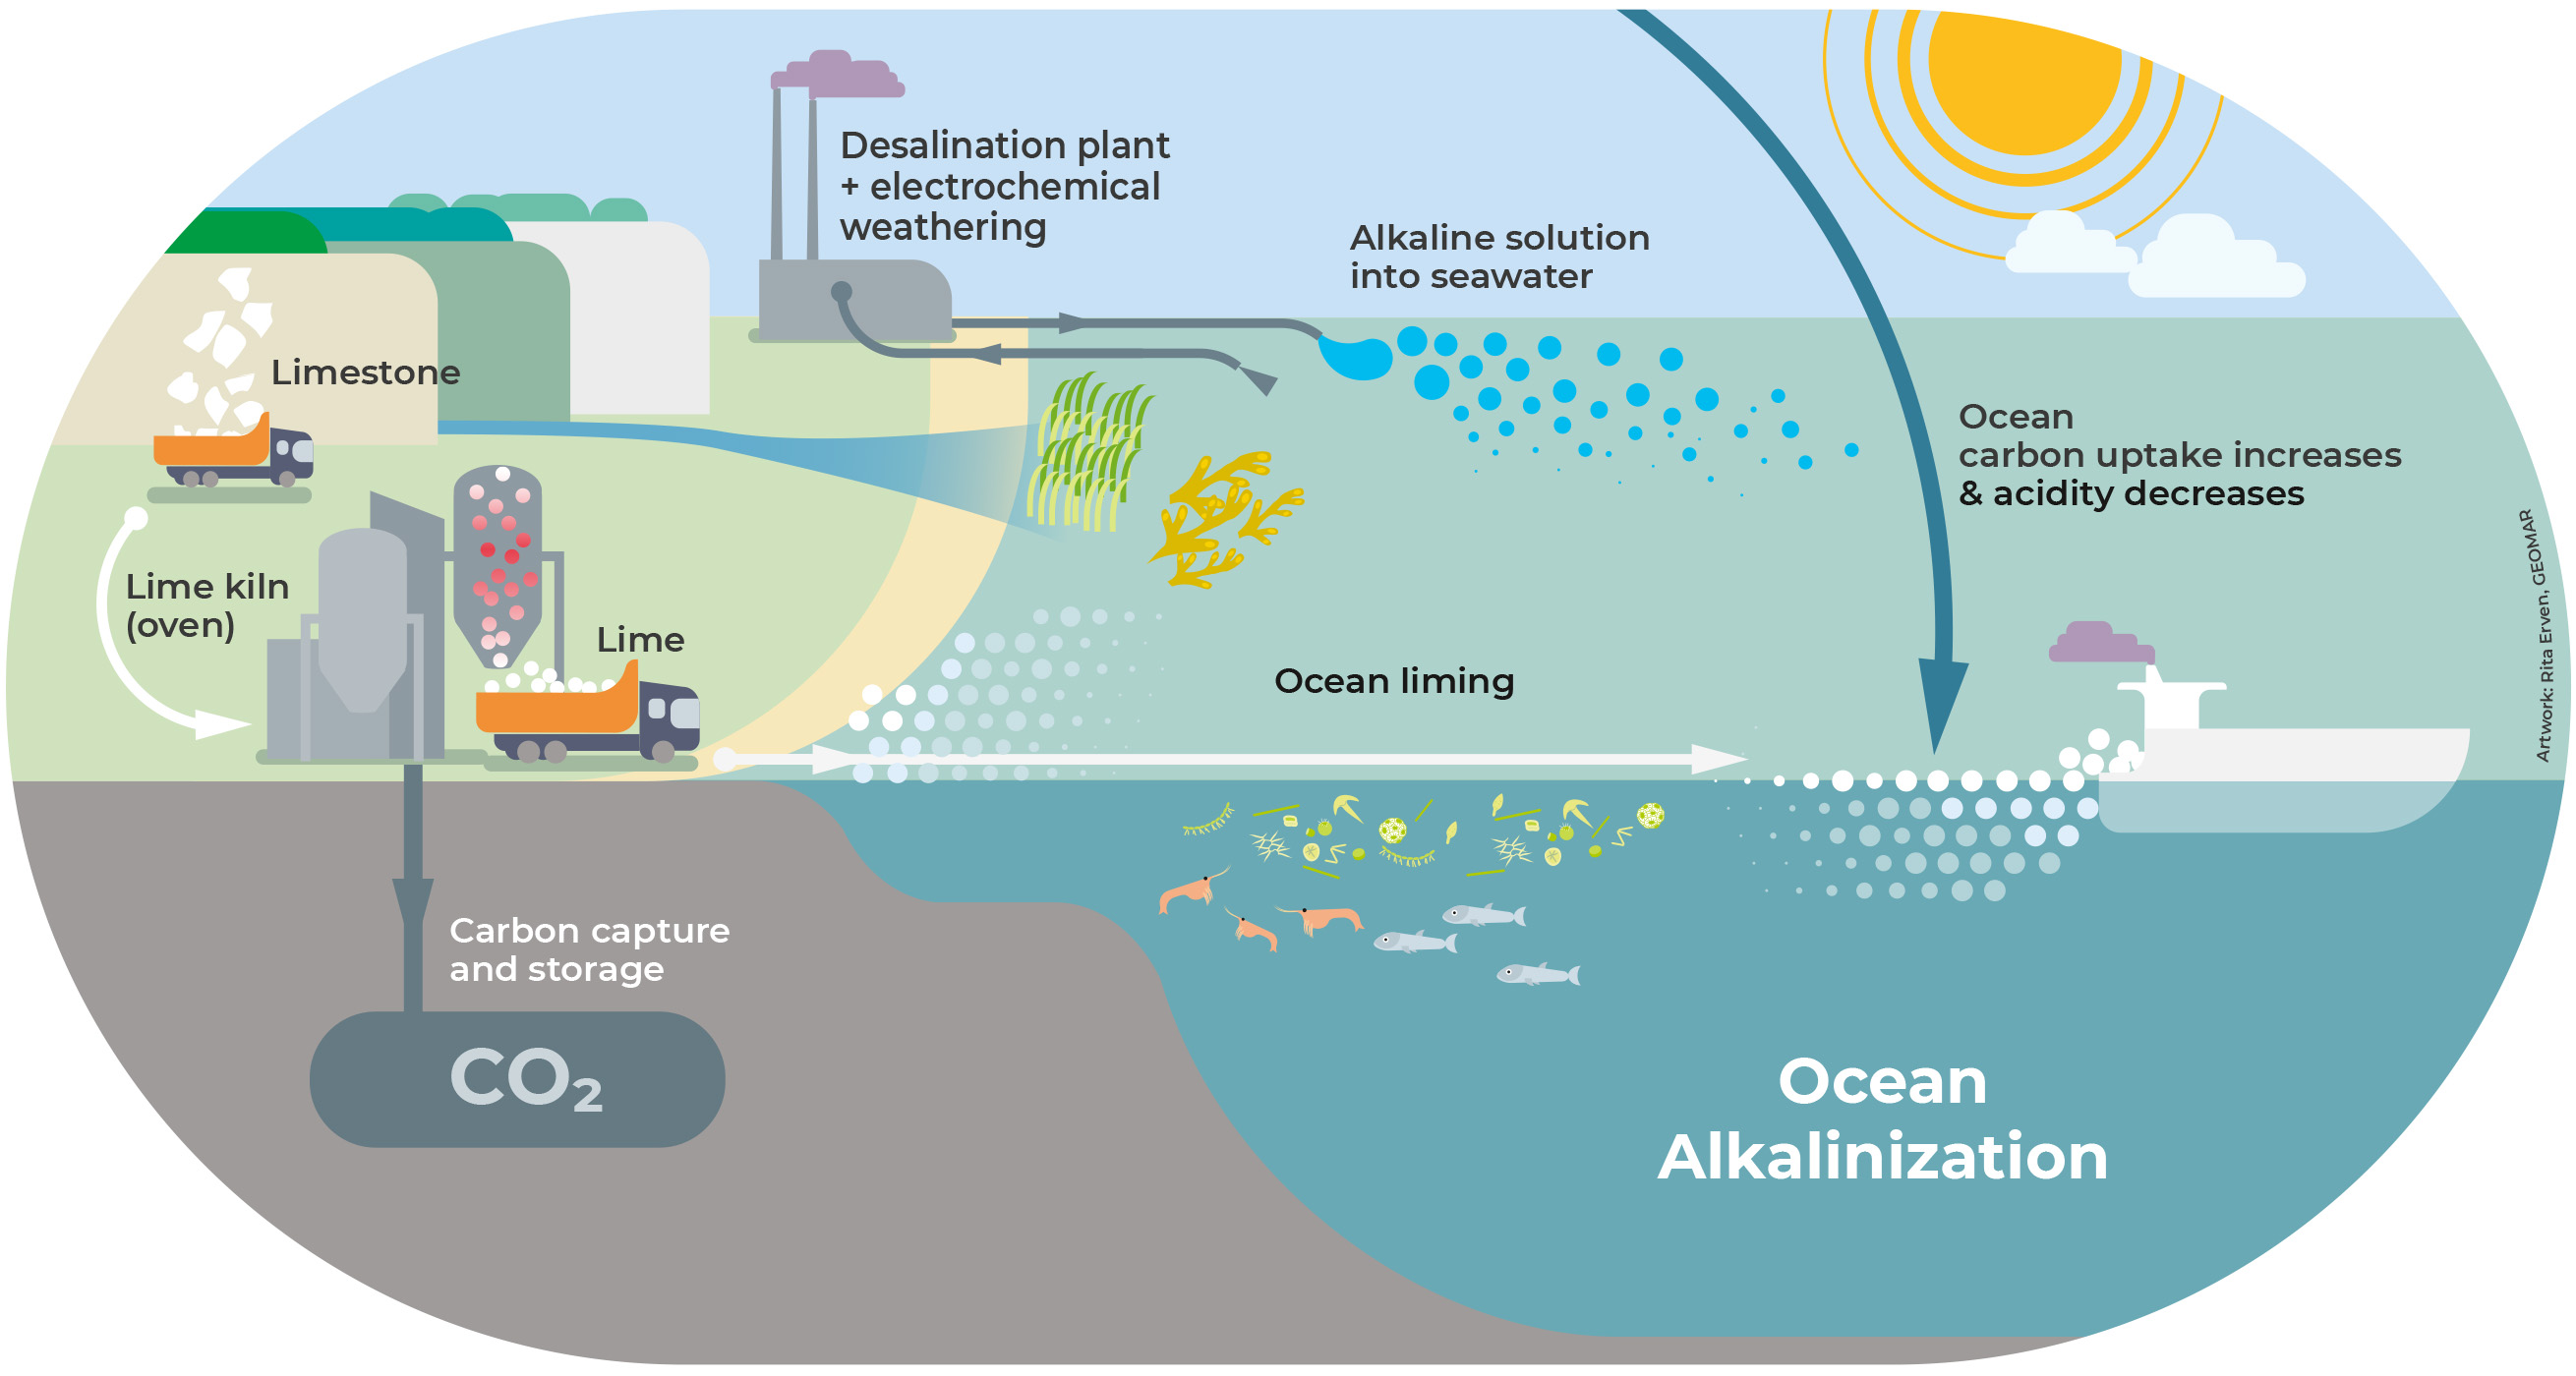
\includegraphics[width=12cm]{fig/1_Introduction/alkalinization_210325.jpg}

\scriptsize Source: Rita Ervin, GEOMAR
\end{figure}

The second method for alkalinity addition is through \acl{oae}, described in \cref{oae}. As atmospheric \ch{CO2} easily dissolves in seawater under the chemical reactions discussed above, \ac{oae} aims to reduce the fragment of aqueous \ch{CO2} present in seawater, which is constantly being exchanged with the atmosphere, and convert it into \ch{HCO3-} and \ch{CO3^{2-}}, thus promoting atmospheric \ch{CO2} drawdown. 

In general terms, \ac{oae} involves the dissolution of silicate and carbonate rocks and solutions, by either grinding and dispersal on the ocean surface, or by electro-chemical reaction on land-based stations or on board of ships. To mention a few, alkalinity can be generated through calcium carbonate dissolution, which produces carbonate ions (see \ref{split}) \citep{rau2008electrochemical}, or by converting salt present in seawater or desalination plants into a basic solution (see \ref{electrochem}) \citep{shaw2022understanding}. The product of such reactions, that is, alkalinised seawater, would then be returned to the ocean to increase its buffering capacity.

\begin{center}

\begin{equation}
\label{split}
\ch{CaCO3} \leftrightarrow \ch{Ca}\textsuperscript{2+} + \ch{CO3}\textsuperscript{2-}
\end{equation}

\begin{equation}
\label{electrochem}
\ch{NaCl} + \ch{H2O} \leftrightarrow \ch{HCl} + \ch{NaOH}
\end{equation}

\end{center}

At present day, natural ocean weathering already sequesters around 0.5 billion tonnes of \ch{CO2} every year \citep{NAP26278}.

\subsection[\texorpdfstring{OAE}{OAE}-induced impacts:]{\ac{oae}-induced impacts:}

\ac{oae} induces ocean \ch{pCO2} to decrease as seawater chemistry moves towards a carbonate-dominated system. This shift drives the \ac{dic} pool to be depleted in \ch{CO2}(aq), leading to more \ch{CO2} to flow from the atmosphere into the ocean to restore the air-sea equilibrium. Due to its properties, alkalinity addition is therefore strictly linked to the replenishment of the \ac{dic} pool \citep{he2022limits}.

\ch{CO2} uptake efficiency varies depending on the amount of alkalinity needed to drive such alterations. This principle is expressed by the \ac{rf}, which defines \ch{pCO2} sensitivity as a function of \ac{dic} variations. \ac{rf} is mathematically translated as the relative change in \ch{pCO2} divided by the relative change in \ac{dic} \citep{devries2022ocean} and it is inversely proportional to the ocean's buffering capacity \citep{renforth2017assessing}. Higher (lower) \ac{rf} implies that smaller (larger) \ac{dic} modulations are needed to produce the same ocean \ch{pCO2} response. It has been estimated that, in a global range between 8 and 15, \ac{rf} has risen by one unit since pre-industrial levels \citep{mcneil2019changing, egleston2010revelle}.

As \ac{oae} aims to enlarge the air-to-sea \ch{CO2} disequilibrium, it is worth highlighting the main properties that regulate the requilibration timescale which, as cited in \cite{jones2014spatial}, is seasonally and location dependent, varying from a few months to over a year. Generally speaking, the \ch{CO2} requilibration rate ($\tau$\ch{CO2}) is determined by four factors (\ref{equilrates}): 

\begin{center}

\begin{equation} 
\label{equilrates}
\tau \ch{CO2} = hR/GB
\end{equation}

\end{center}

where h is the \ac{mld}, R is the \ch{CO2}(aq):\ac{dic} ratio, G is the gas transfer velocity, and B is the \acl{rf}. From this equation, it is derived that locations with shallower \ac{mld} will allow for faster requilibration, given its linear relation with the \ch{CO2}(aq) content. G is driven by, among others, wind-induced turbulence, and areas exposed to high wind speed will experience faster requilibration. At the same time, however, wind speed deepens the \ac{mld} and slows down the exchange rate, so that the dominating process will drive the transfer rate. Whereas R usually decreases with latitude, B has the opposite trend and, inversely correlated with $\tau$ \ch{CO2}, shortens the gas exchange rate \citep{jones2014spatial}. 

\ac{oae} has the additional benefit of alleviating the ocean from increasing acidification, a present-day threat that relates to rising \ch{H+} concentration in seawater as a consequence of \ch{CO2} downward inputs \citep{ma2015primary}. Since the start of the \ac{ir}, ocean pH has declined by 0.1 units \citep{devries2022ocean}, leading to widespread impacts on the ocean biota such as major coral bleaching events and reduced biodiversity.

\begin{figure}[H]
\caption{Relation between ocean carbon chemistry and pH}
\label{pHacid}
\centering
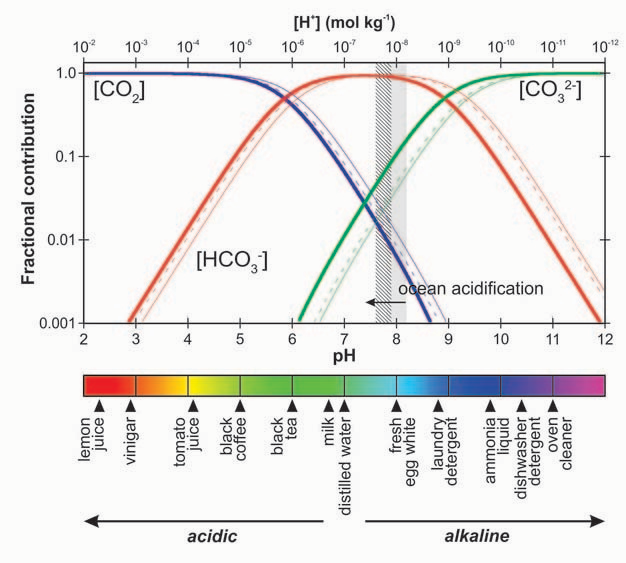
\includegraphics[width=10cm]{fig/1_Introduction/Carbonate_Chemistry.png}

\scriptsize Source: \cite{barker2012ocean}
\end{figure}

\Cref{pHacid} represents the relation between pH and ocean chemistry. Each coloured line describes the concentration of the three forms of carbon as a function of pH. At higher pH, possibly induced by \ac{oae}, the system moves towards a carbonate-dominated environment (green line in \Cref{pHacid}), where more carbonate ions are available and aqueous \ch{CO2} content drops. Moving towards the left-hand side of the graph, when pH lowers, carbon present in the form of \ch{CO2}(aq) grows, whereas the concentration of its stable forms decreases.

pH is partly affected by the biological carbonate counter-pump, which regulates the formation and dissolution of \ch{CaCO3}. pH neutralisation happens when, as a surplus quantity of \ch{CO2} enters the system, carbonate ions bond with extra \ch{H+} to form bicarbonates and reduce acidity \citep{scott2019role, barker2012ocean}. At the same time, however, \ch{CO3^{2-}} that combines with calcium (\ch{Ca}\textsuperscript{2+}) to build the exoskeletons of marine calcifiers, starts dissolving to favour bicarbonate production \citep{mcnicholl2020ocean}.

\subsection[Limitations and challenges of \texorpdfstring{OAE}{OAE}]{Limitations and challenges of \ac{oae}:}

\ac{oae} bears multiple challenges and uncertainties on costs, logistics and environmental repercussions. Most minerals, although abundant on the earth's crust, are not readily soluble in seawater, or can be only under specific physical conditions \citep{kheshgi1995sequestering}. In most approaches, \ac{oae} would therefore entail mineral extraction, processing and transportation, which would demand economic funding, energy consumption and logistical monitoring \citep{NAP26278}. 

The location and physical properties of the injection site also matter: the \ac{mld}, the surface water mean residence time and local ocean circulation patterns all have an effect on air-sea equilibration rates, and therefore on the efficacy of this technique \citep{wang2023simulated, he2022limits}. Decreased, particle size is another important feature to enhance dissolution and further \ch{CO2} uptake from the ocean surface. Lastly, the frequency and periodicity of deployment influences \ac{oae} efficiency, leading to the investigation of methods such as continuous alkalinity addition or in pulses, and addition to the open ocean or near the coast \citep{NAP26278}.

The biotic impacts of alkalinity addition are concerning. The utilisation of silicates, for example, could intensify fertilisation due to iron-rich mineral dissolution, which would in turn increase the production of other potent \ac{ghg} \citep{renforth2017assessing}. Dropping \ch{CO2} concentration could also lead to respiratory alkalosis, already observed in previous experiments \citep{cripps2013biological}. The distribution of certain rocks would release elements like nickel which, in large quantities, could be toxic to the \ac{pp} exposed to these particles. This could lead to bio-accumulation and bio-magnification throughout the trophic chain, with potentially dangerous repercussions on biodiversity and food security. 

pH and aragonite saturation state levels, which defines the threshold for carbonate dissolution, are expected to rise substantially with \ac{oae} application, especially close to the injection site or in areas with already elevated alkalinity levels. This could possibly lead to oversaturation above present-day values, which would consume alkalinity through spontaneous abiotic and secondary calcification, and reverse the desired objectives \citep{NAP26278, de1984ph}.

The socio-economic and legal uncertainties posed by \ac{oae} are also worth mentioning. If deployed at a large scale, \ac{oae} would require an extensive monitoring and verification programme \citep{ho2023chapter}. Although some tools are already being used to gather ocean data and examine carbon fluxes, these methods are limited in both logistics and resolution. Additionally, recent studies have found that alkalinity enhancement may be associated with a form of marine 'pollution' and 'dumping', as defined by the United Nations Convention on the Law of the Sea and London Convention and Protocol, respectively \citep{NAP26278}.

\section{Seasonal air-sea \ch{CO2} exchange:}

Seasonality is a fundamental property of the annual net carbon cycle \citep{rodgers2023seasonal, fassbender2022quantifying}. The impacts of increasing anthropogenic emissions on the seasonal cycle of \ch{CO2} and ocean \ch{pCO2}, and more broadly on the ocean biochemistry, have been largely investigated \citep{lerner2021drivers, landschutzer2018strengthening, kwiatkowski2018diverging}, leading to the conclusion that higher atmospheric \ch{CO2} concentration will alter seasonal extremes in all ocean regions \citep{landschutzer2018strengthening}. This will most likely take place because the system will experience an enhanced sensitivity to the thermal component that regulates \ch{CO2} variability \citep{mcneil2019changing}. The ocean will therefore become more vulnerable to minimal perturbations, although with geographical and temporal variations \citep{landschutzer2018strengthening, egleston2010revelle}.

Seasonally, ocean \ch{CO2} flux and \ch{pCO2} are controlled by two main factors: \ac{sst} and \ac{dic}. Especially on the short term, \ac{sst} acts on the solubility of gases in seawater. In summer months, warm water leads to decreased solubility and \ch{CO2} outgassing, whereas colder and saltier water in winter favours solubility and \ch{CO2} uptake \citep{williams2011ocean}. On the other hand, \ac{dic} concentration is a function of, among others, \ac{om} production and respiration, water upwelling and downwelling, calcification and dissolution. In winter, where processes like upwelling and \ac{om} respiration prevail, the ocean will easily lose \ch{CO2} to the atmosphere, whereas summertime \ac{om} production and downwelling will favour atmospheric \ch{CO2} drawdown.

Temperature and \ac{dic} concentration influence seasonal variability at different scales and magnitudes, making it geographically dependent. As the dynamics of these two processes oppose each other \citep{lerner2021drivers, takahashi2002global}, the one prevailing will drive the direction of seasonal \ch{CO2} exchange at that location \citep{sarmiento2006ocean}. Generally, latitudes higher than 40\textdegree{} are more affected by the non-thermal component, namely \ac{dic} concentration, whereas the opposite happens for latitudes below 40\textdegree{}, where the thermal component dominates \citep{mcneil2019changing, gallego2018drivers, sarmiento2006ocean}. Counter-intuitively, seasonality at the equator is driven by the non-thermal component, due to the higher \ch{CO2}(aq) to \ac{dic} ratio than its neighbouring areas \citep{fassbender2017nonuniform}. 

This explains why the ocean generally operates in a reversed pattern at different latitudes. Higher than 40\textdegree{} and at the equator, it acts as a \ch{CO2} sink in summer, mainly due to high photosynthetic activity in the blooming season, and as a source in winter, due to upwelling and \ac{om} respiration \citep{gallego2018drivers, takahashi2002global}. Conversely, at latitudes lower than 40\textdegree{}, the ocean acts as a \ch{CO2} source (sink) in summer (winter) when solubility decreases (increases) \citep{yun2022enhance}. A recent study by \cite{lerner2021drivers} brings an additional distinction of the sub-polar regions, whose \ch{CO2} seasonality is equally influenced by the two factors.

Like air-sea gas transfer, ocean \ch{pCO2} undergoes seasonal variability which is non-uniform to temperature and \ac{dic} throughout the ocean. \ac{rf} is strictly related to alkalinity and to the ocean buffering capacity \citep{egleston2010revelle}. Generally, larger \ac{rf} values are found at higher latitudes, where small changes in \ac{dic} cause large \ch{pCO2} modulations, whereas \ac{rf} becomes lower and lower as one approaches the tropics, where temperature controls \ch{pCO2} variability over \ac{dic} fluxes \citep{fassbender2018seasonal}. 

\subsection{Climate change impacts on \ch{CO2} seasonality:}

Rising \ch{CO2} concentration, both in the atmosphere and in the ocean, tends to affect the amplitude of its seasonal flux, defined in this manuscript as the difference between the annual maximum and the annual minimum. In general terms, ocean \ch{CO2} seasonality is enhanced at latitudes higher than 40\textdegree{} and depressed at latitudes lower than 40\textdegree{} \citep{yun2022enhance}. This is confirmed by both observations and model simulations, which show a larger \ch{pCO2} amplitude in polar and sub-polar areas than towards the equator \citep{schwinger2022report, gallego2018drivers}. 

As the ocean is closely linked to the terrestrial carbon cycle, which provides large quantities of carbon via land runoff, climate-induced changes to terrestrial patterns will play a fundamental role in regulating future \ch{CO2} seasonality in seawater. Land processes like plant photosynthesis and soil respiration are expected to undergo strong temperature-driven seasonal variations, triggered by its increased system vulnerability, which will in turn affect all ocean regions \citep{liu2017seasonal}. 

Given the mechanisms described in the previous section, the projected soaring of \ac{sst} induced by global warming will trigger opposing regional reactions of the \ch{CO2} seasonal cycle. Location South of 40\textdegree{}, where seasonality is driven by temperature, will become more sensitive to thermal variations, leading to an amplification signal. The opposite pattern, thus an amplitude compression, will affect latitudes North of 40\textdegree{}, where biophysical processes will be compensated for by \ac{sst}-driven effects. Additionally, it was found that, in winter, the effects of high wind speed and a deeper mixed layer will outcompete those in summer. This will lead to an amplification of the flux that is dominating in cold months, hence outgassing towards the poles and ingassing towards the tropics \citep{fassbender2022quantifying}. 

With global warming, pH seasonality is also expected to vary. Although the amount of hydrogen ions in the ocean will rise due to increasing \ch{CO2} uptake from the atmosphere, a negative correlation has been registered between pH seasonality and annual proton concentration, whereby the estimated annual increase in hydrogen ions in seawater will be greater relative to its seasonal growth. Consequently, higher \ch{CO2} flux into the ocean, and thus higher \ch{H+} content, will have a compressing effect on the seasonal pattern of pH in seawater \citep{kwiatkowski2022modified, kwiatkowski2018diverging}. 

\subsection{\ch{CO2} seasonality in the study area:}

This section gives an overview of the main physical and biological properties that characterise \ch{CO2} seasonality in the study area, setting the initial conditions from which this analysis begins. The focus is on the North Sea as, although the experiment area stretches further, it will be shown that, in that region, alkalinity addition has a predominant impact. 

In previous research, locations like the study area, which covers a regional sea and a continental shelf, have notoriously been neglected in the quantification of global ocean \ch{CO2} uptake \citep{prowe2009mechanisms, borges2006carbon}. However, recent studies highlighted an expanding interest in understanding their key role in the air-sea \ch{CO2} fluxes, both seasonally and inter-annually \citep{omar2010spatiotemporal}. These regions portray a dynamic biological activity and they contribute about 20\% to the ocean's annual anthropogenic \ch{CO2} uptake \citep{thomas2004enhanced}. This realisation led to the theory of the continental shelf pump as that mechanism in which marginal and shoreline seas transfer atmospheric \ch{CO2} to the subsurface and then to the open ocean \citep{salt2013variability, bozec2005continental, thomas2004enhanced}. In the examined case, the North Sea serves as connection between the European coastline and the North Atlantic. 

The air-sea \ch{CO2} flux in the North Sea is characterised by a strong North-to-South seasonal gradient \citep{salt2013variability, prowe2009mechanisms}. Biological drivers dominate in the well stratified northern North Sea (A of \cref{dsmw}), where a relatively shallow mixed layer allows for nutrient-rich waters to stay at the surface and encourage phytoplankton bloom during the productive season (C of \cref{dsmw}). \ac{om} that there accumulates then sinks below the mixed layer, where remineralisation can happen far from atmospheric contact. \ch{CO2} sequestration through carbon fixation hence outweighs temperature-driven ocean \ch{pCO2} increase, making the area a strong carbon sink \citep{prowe2009mechanisms}. 

\begin{figure}[H]
\caption[Latitudinal transect of the North Sea for the baseline seasonal cycle of \texorpdfstring{DIC}{DIC}, \texorpdfstring{SST}{SST}, \texorpdfstring{MLD}{MLD}, and wind speed averaged over 2015-2100 in SSP1-2.6.]{From left to right, latitudinal transect of the North Sea for the baseline seasonal cycle of \ac{dic} (A), \ac{sst} (B), \ac{mld} (C), and wind speed (D) averaged over 2015-2100 in SSP1-2.6.}
\label{dsmw}
\centering
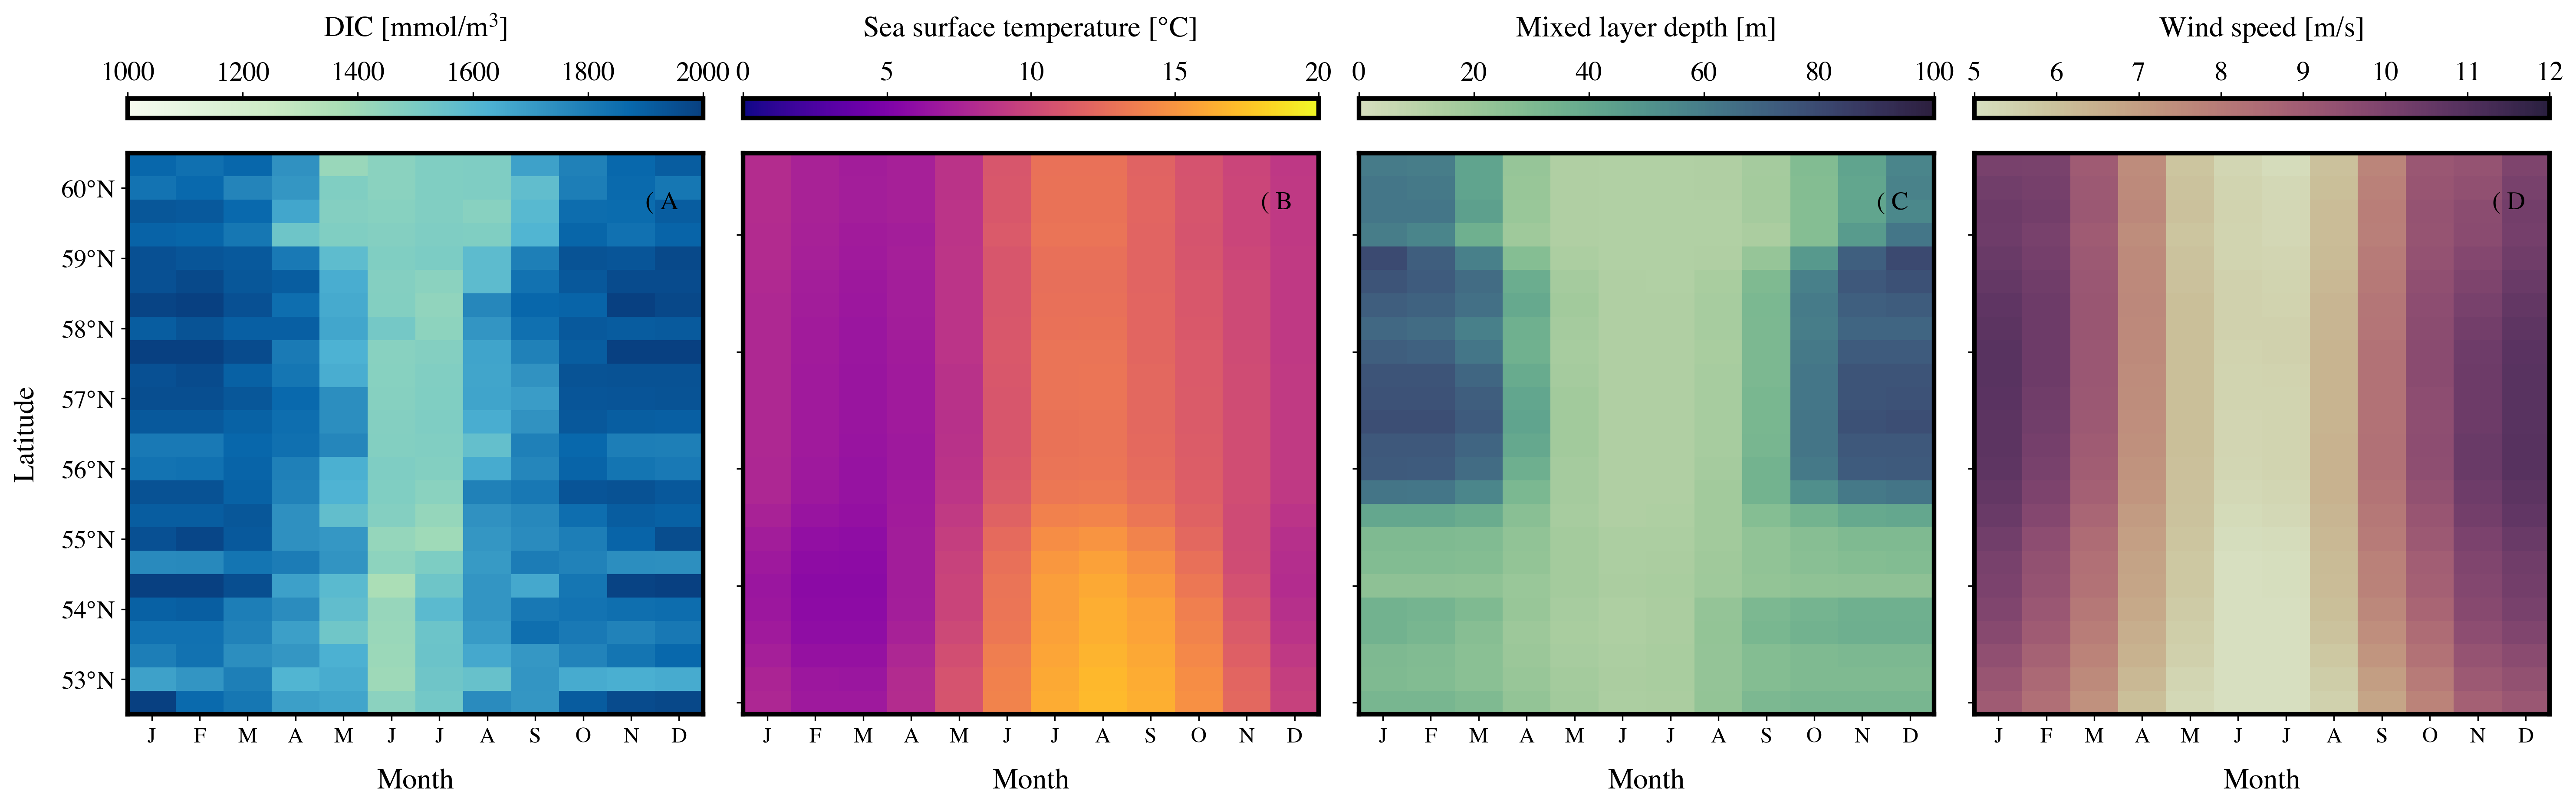
\includegraphics[width=15cm]{fig/1_Introduction/dsmw.png}

\end{figure}

On the other hand, in the southern North Sea and the adjacent European continental shelf, where high wind speed (D of \cref{dsmw}) and shallow water depth (C of \cref{dsmw}) generate a more uniform layer all year round \citep{thomas2009enhanced}, the air-sea \ch{CO2} exchange is mainly induced by temperature variability (B of \cref{dsmw}) \citep{salt2013variability}. Due to a shallow water column, carbon production and remineralisation happen within the same surface compartment, where \ch{CO2} can easily be transferred with the atmosphere \citep{prowe2009mechanisms, thomas2004enhanced}. Thus, community respiration outweighs \ac{pp}-driven photosynthesis \citep{artioli2012carbonate} and this area constitutes a weak \ch{CO2} source to the atmosphere \citep{prowe2009mechanisms}. 

\ch{pCO2} seasonality in the North Sea follows a well-established pattern induced by its two biogeochemical provinces defined above. The summer season is where this divide is most evident, as the spring bloom of \ac{pp} in the northern region poses the conditions for a strong \ch{CO2} undersaturation in the surface layer, whereas subsurface biological respiration enhances the \ac{dic} pool far from the atmosphere. Conversely, the southern North Sea quickly becomes oversaturated with respect to surface \ch{CO2} content owing to the slowdown of \ac{pp} and temperature rise \citep{thomas2004enhanced}. 

In marginal seas like the North Sea, alkalinity seasonality remains relatively homogeneous. Especially in the southern, shallower waters, the seasonal cycle of alkalinity is a combination of a multitude of physical and biological interactions. Among others, the most important sources of alkalinity are runoff and water-sediment relations \citep{omar2010spatiotemporal}, together with the anaerobic degradation of \ac{om}, especially in the Wadden Sea. In general terms, this results in highest alkalinity levels in summer and lowest in winter \citep{thomas2009enhanced}. 

Additionally, a 2013 study on the waterway contribution of alkalinity in the southern North Sea revealed that river loads of nutrients have a relatively small impact on the observed alkalinity due to low concentrations in the Elbe river. On the other hand, the Wadden Sea holds a remarkable 68\% contribution to annual alkalinity levels in the region \citep{schwichtenberg2013drivers}. 

pH is intrinsically connected to the processes described above. In the northern North Sea, more biologically active, \ch{CO2} export at the surface layer maintains a relatively high pH, while \ac{om} respiration in southern waters triggers pH decline \citep{salt2013variability, thomas2004enhanced}. Whereas this pH divide is hardly detectable in winter, a strong North-to-South gradient is registered in summer: southern water pH is reduced whereas northern pH is enhanced \citep{thomas2009enhanced}. 

